% ============================================================
% ============================================================
%  DROPLET IMPINGEMENT
% ============================================================
% ============================================================

\section[Impingement]{\textbf{Droplet Impingement}}

% ============================================================
%  Water Mass Grid Convergence
% ============================================================

\begin{frame}{\small  Water Mass Grid Convergence (15 Bins)}
\scriptsize

\begin{columns}[T,onlytextwidth]

\begin{column}{0.50\textwidth}
    \centering
    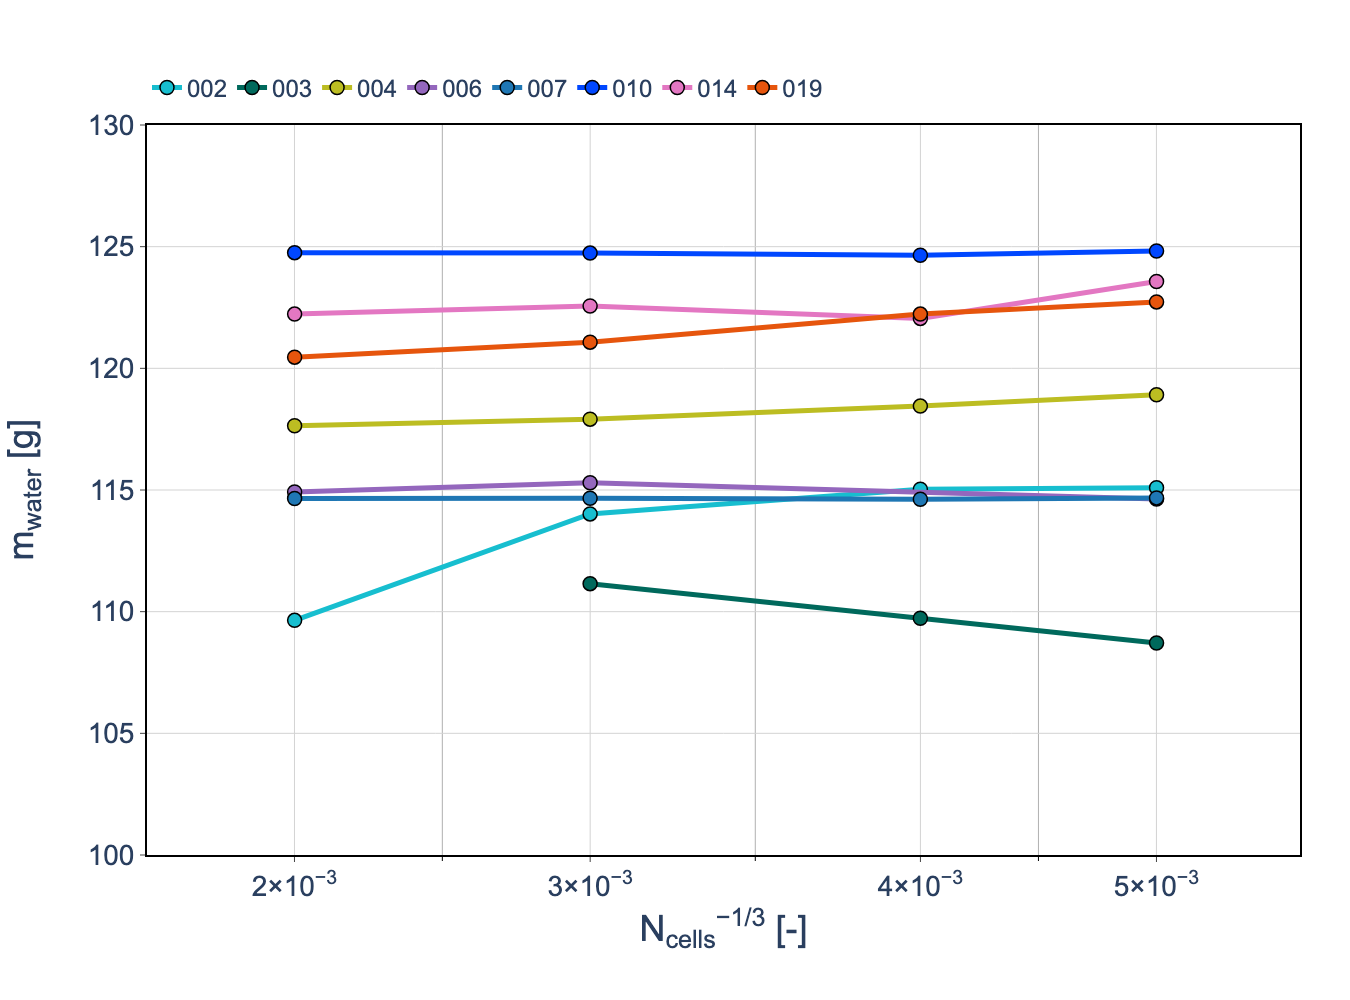
\includegraphics[trim={0cm 1cm 1cm 2.6cm}, clip, width=0.98\textwidth]{FIGURES/IMPINGEMENT/tc_naca0012_ae3932_water_mass_vs_n_unspecified_bins15_all_grid_levels.png}
    \textbf{Grid-Level Values}
    \vspace{0.05cm}
\end{column}

\begin{column}{0.50\textwidth}
    \centering
    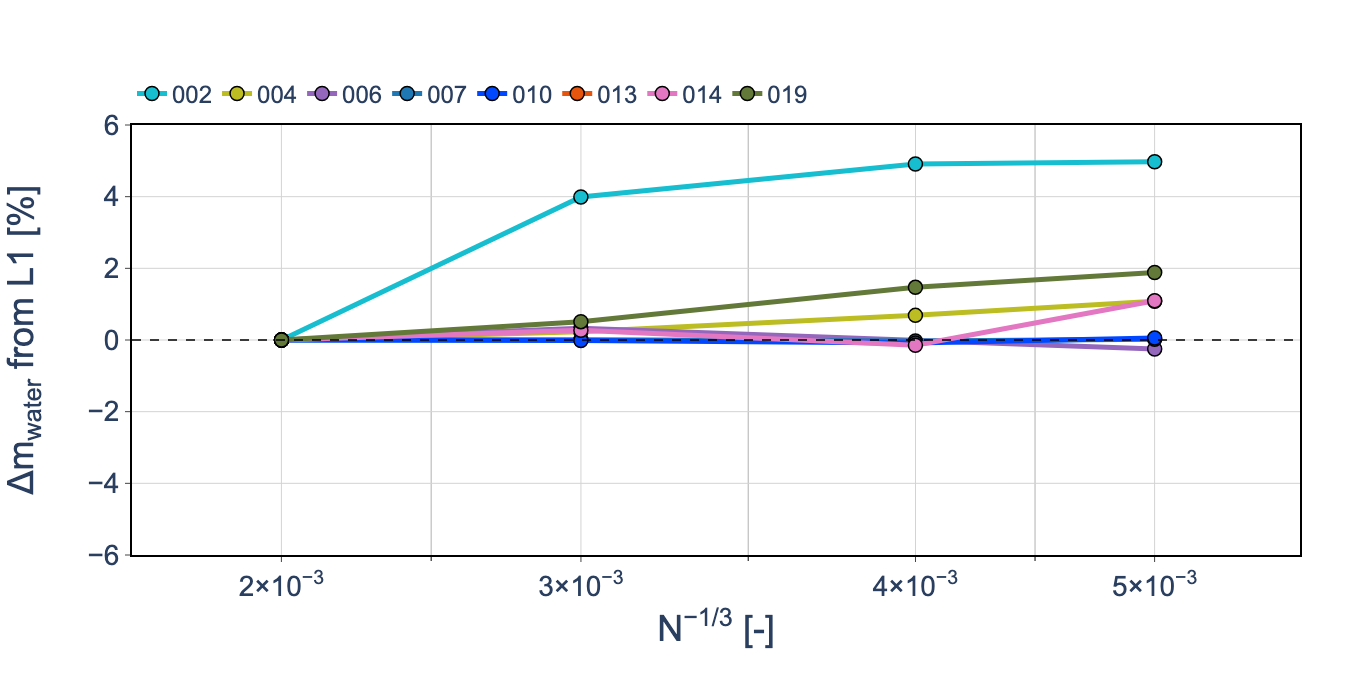
\includegraphics[trim={0cm 1cm 1cm 2.6cm}, clip, width=0.98\textwidth]{FIGURES/IMPINGEMENT/tc_naca0012_ae3932_water_mass_vs_n_unspecified_bins15_all_grid_levels_relative_to_l1.png}
    \textbf{Relative to L1}
    \vspace{0.05cm}
\end{column}

\end{columns}

\vspace{-0.15cm}

\begin{block}{\scriptsize Observations}
\begin{itemize}
    \item For the 15-bin distribution, the L1 median impinged water mass is $119.05~\mathrm{g}$, with an IQR of $6.39~\mathrm{g}$ ($5.37\%$).
    \item Most submissions exhibit weak grid sensitivity and remain close to their L1 prediction across the grid hierarchy.
\end{itemize}
\end{block}

\end{frame}


% ============================================================
%  Droplet Distribution Sensitivity
% ============================================================

\begin{frame}{\small  Droplet Distribution Sensitivity (L1)}
\scriptsize

\vspace{-0.15cm}

\begin{columns}[T,onlytextwidth]

\begin{column}{0.50\textwidth}
    \centering
    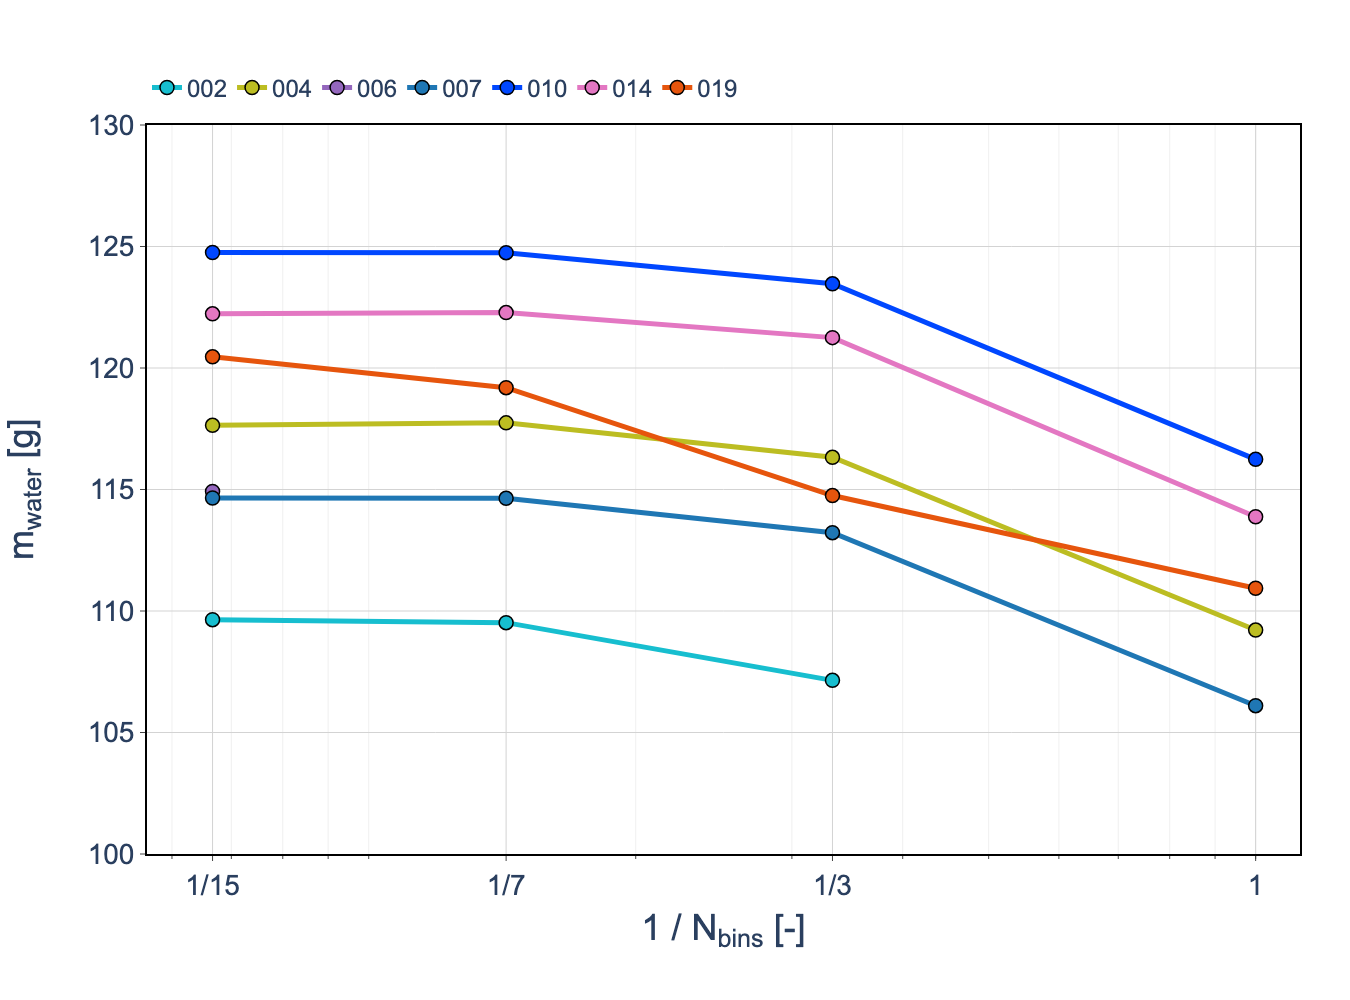
\includegraphics[trim={0cm 1cm 1cm 2.6cm}, clip, width=0.98\textwidth]{FIGURES/IMPINGEMENT/tc_naca0012_ae3932_water_mass_vs_n_unspecified_l1_vs_inverse_bins.png}
    \textbf{Bin-Distribution Values}
    \vspace{0.05cm}
\end{column}

\begin{column}{0.50\textwidth}
    \centering
    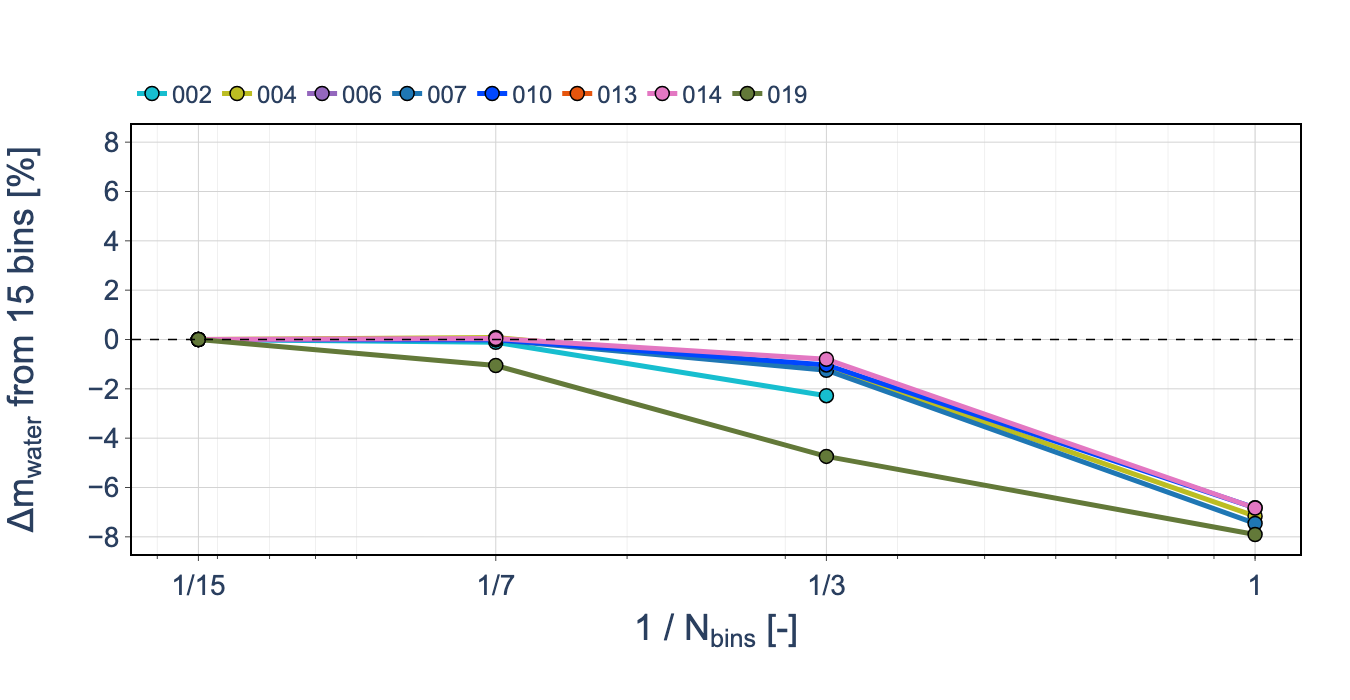
\includegraphics[trim={0cm 1cm 1cm 2.6cm}, clip, width=0.98\textwidth]{FIGURES/IMPINGEMENT/tc_naca0012_ae3932_water_mass_vs_n_unspecified_l1_vs_inverse_bins_relative_to_bins15.png}
    \textbf{Relative to 15 Bins}
    \vspace{0.05cm}
\end{column}

\end{columns}

\vspace{-0.15cm}

\begin{block}{\scriptsize Observations}
\begin{itemize}
    \item The 15- and 7-bin distributions give similar impinged water masses.
    \item Reducing to 3 bins introduces only modest additional differences.
    \item A single-bin reduces collected water mass by about 5--8\% relative to 15 bins.
\end{itemize}
\end{block}

\end{frame}

% ============================================================
%  Collection Efficiency Profiles
% ============================================================

\begin{frame}{\small  Collection Efficiency (L1, 15 Bins)}
\scriptsize

{\centering
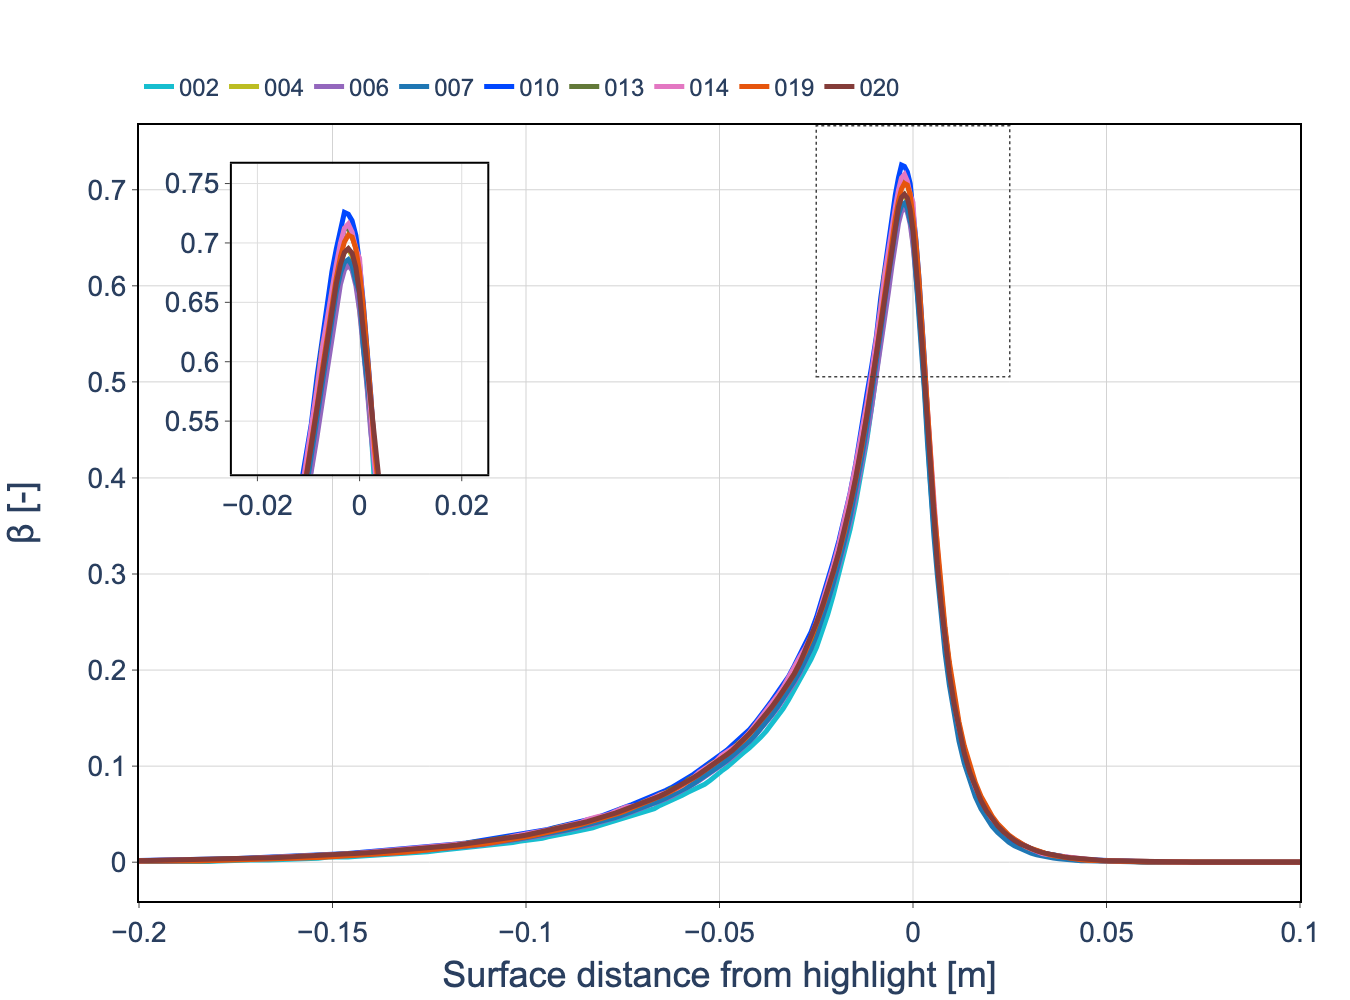
\includegraphics[trim={0cm 0cm 1cm 2.6cm}, clip, width=0.5\textwidth]{FIGURES/IMPINGEMENT/tc_naca0012_ae3932_L1_beta_bins15_vs_s_slice_0p9144_all_roughness.png}

\textbf{Collection Efficiency vs s}
\vspace{0.05cm}
\par}

\begin{block}{\scriptsize Observations}
\begin{itemize}
    \item The L1 collection-efficiency profiles are tightly clustered across submissions and exhibit very similar leading-edge behavior.
    \item Small differences are mainly observed near the peak region and impingement limits.
\end{itemize}
\end{block}

\end{frame}


% ============================================================
% Peak Collection Efficiency -- Grid Convergence
% ============================================================

\begin{frame}{\small Peak Collection Efficiency Grid Convergence (15 Bins)}
\scriptsize

\vspace{-0.3cm}

\begin{columns}[T,onlytextwidth]

\begin{column}{0.50\textwidth}
    \centering
    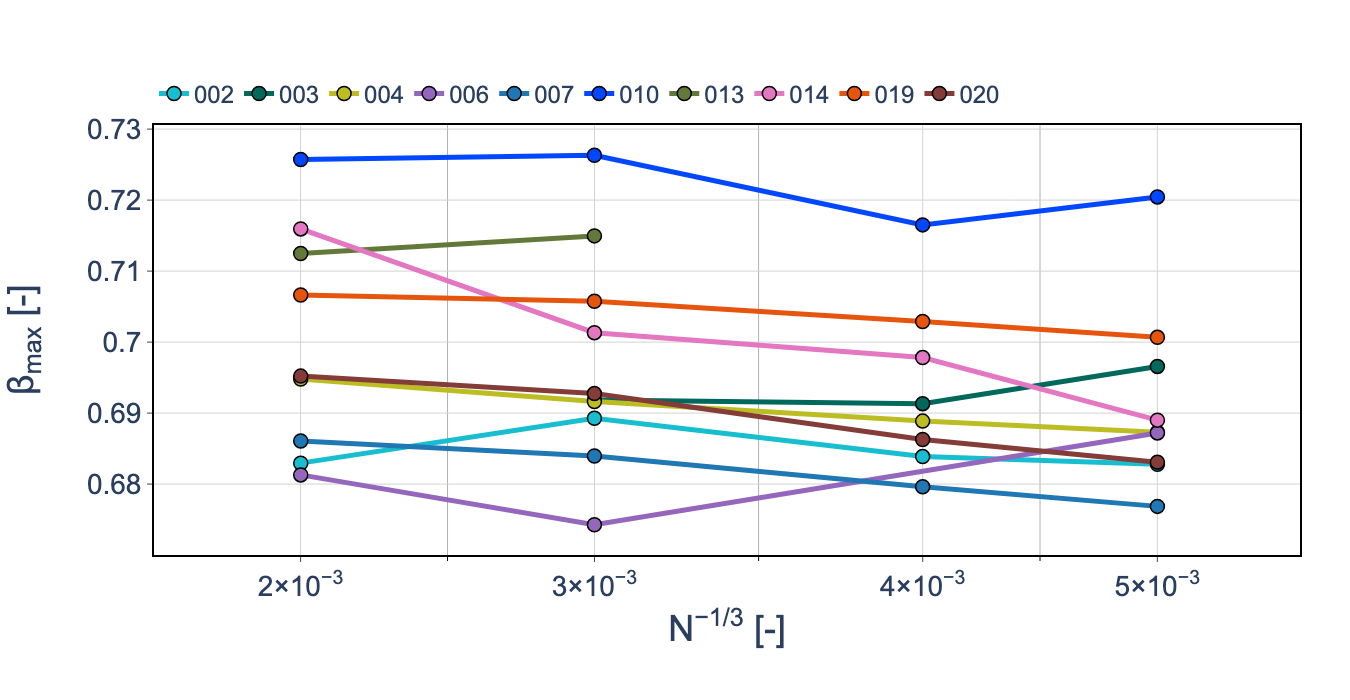
\includegraphics[
        trim={0cm 1cm 1cm 2.6cm},
        clip,
        width=0.98\textwidth
    ]{FIGURES/IMPINGEMENT/tc_naca0012_ae3932_beta_max_bins15.png}

    \textbf{Grid-Level Values}
\end{column}

\begin{column}{0.50\textwidth}
    \centering
    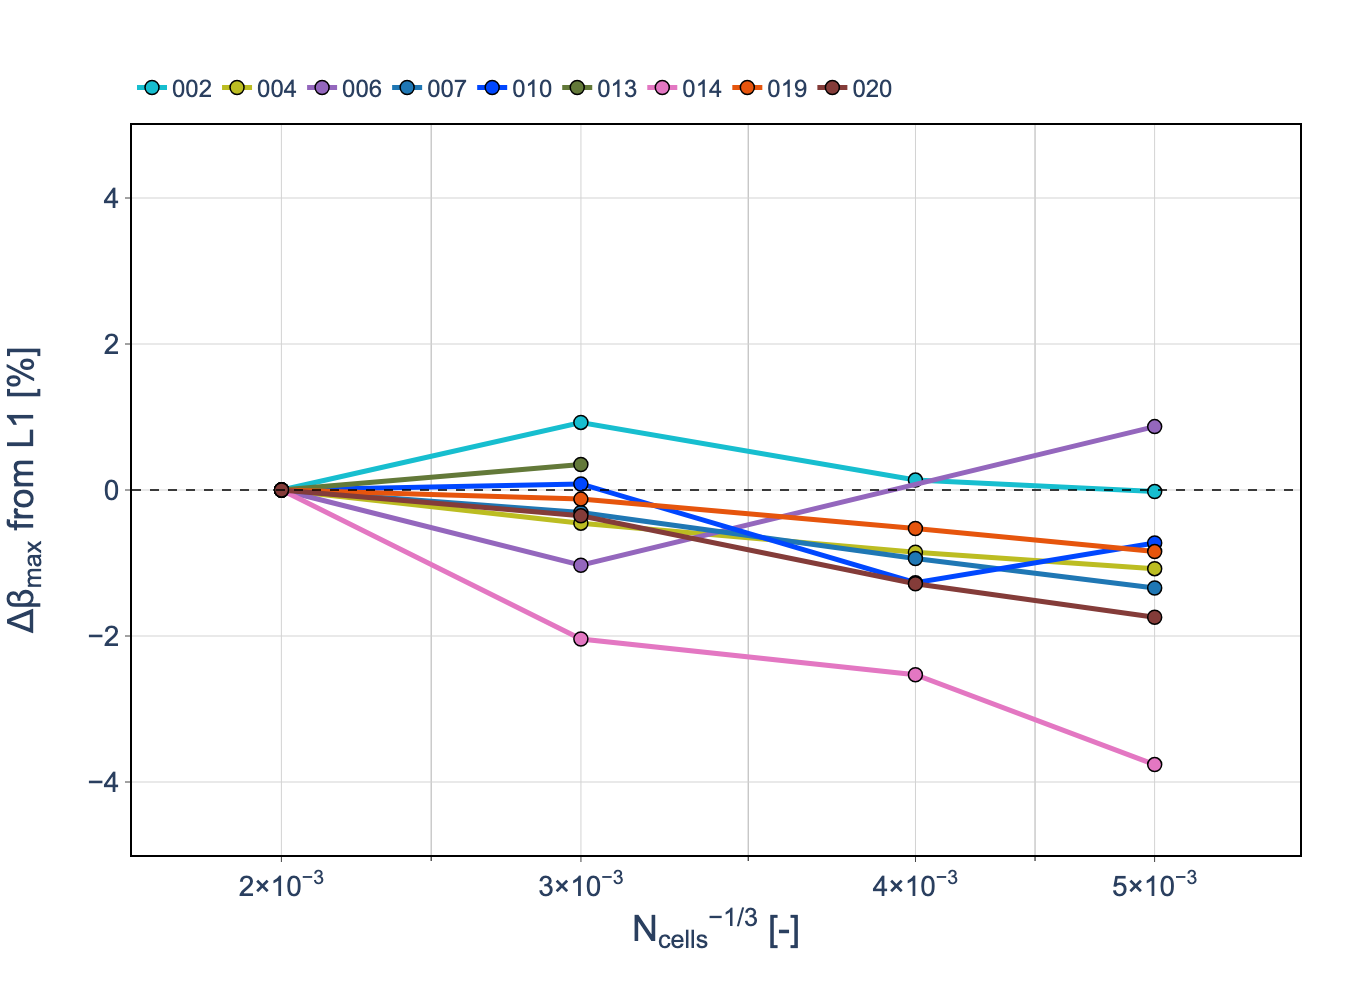
\includegraphics[
        trim={0cm 1cm 1cm 2.6cm},
        clip,
        width=0.98\textwidth
    ]{FIGURES/IMPINGEMENT/tc_naca0012_ae3932_beta_max_bins15_relative_to_l1.png}

    \textbf{Relative to L1}
\end{column}

\end{columns}

\vspace{-0.15cm}

\begin{block}{\scriptsize Observations}
\begin{itemize}
    \item At L1, the median $\beta_{\max}=0.695$ , with a $3.0\%$ IQR.
    \item $\beta_{\max}$ shows limited sensitivity to spatial grid refinement.
\end{itemize}
\end{block}

\end{frame}


% ============================================================
% Peak Collection Efficiency -- Bin Convergence
% ============================================================

\begin{frame}{\small Peak Collection Efficiency Droplet-Bin Convergence (L1)}
\scriptsize

\vspace{-0.3cm}

\begin{columns}[T,onlytextwidth]

\begin{column}{0.50\textwidth}
    \centering
    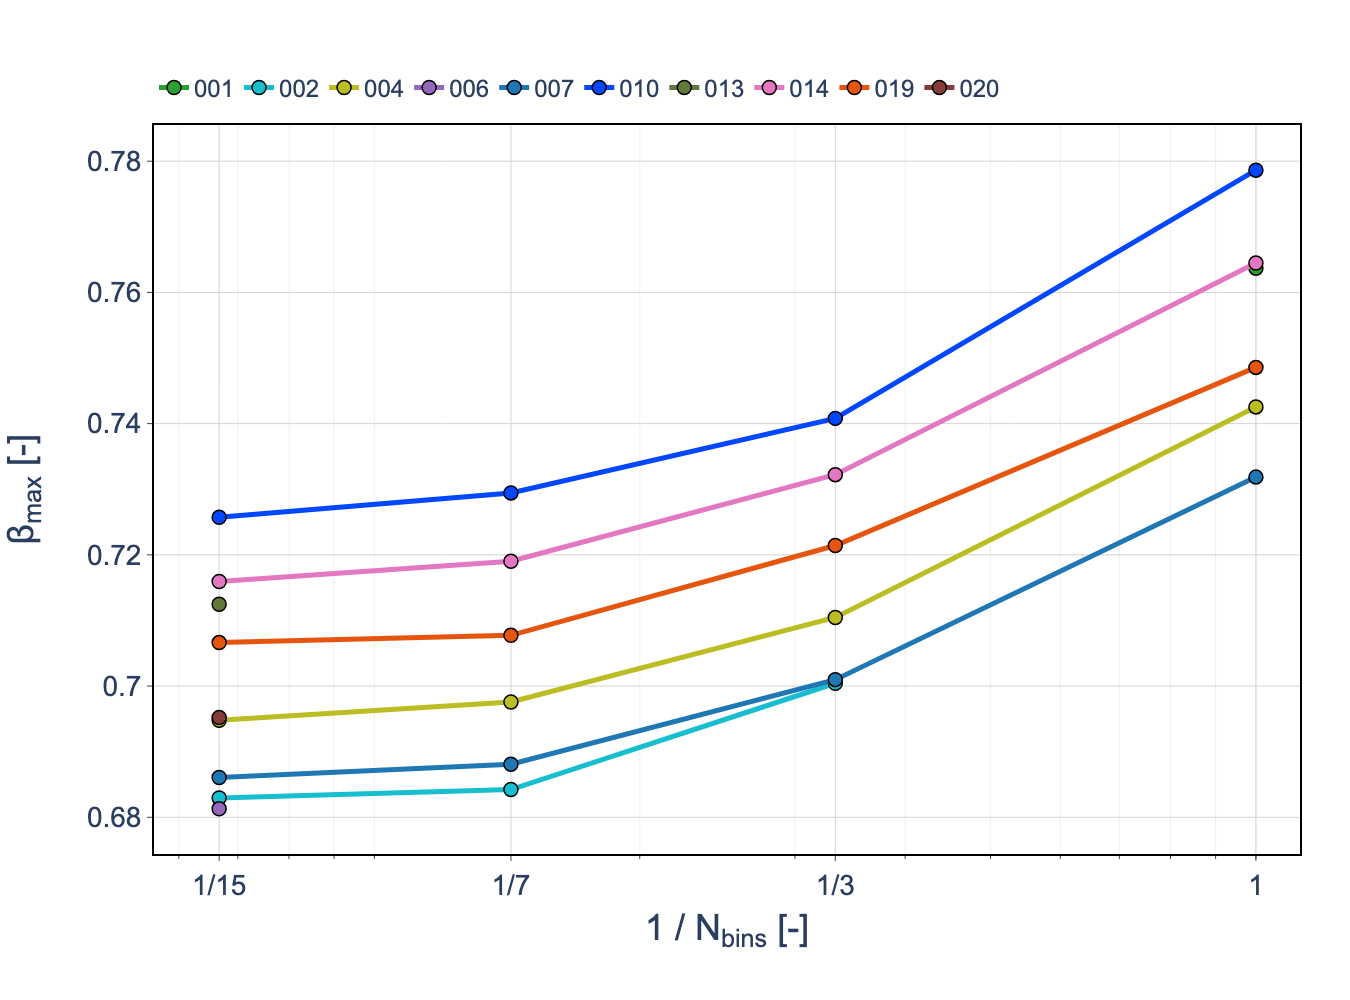
\includegraphics[
        trim={0cm 1cm 1cm 2.6cm},
        clip,
        width=0.98\textwidth
    ]{FIGURES/IMPINGEMENT/tc_naca0012_ae3932_beta_max_distribution_convergence_l1.png}

    \textbf{Bin-Distribution Values}
\end{column}

\begin{column}{0.50\textwidth}
    \centering
    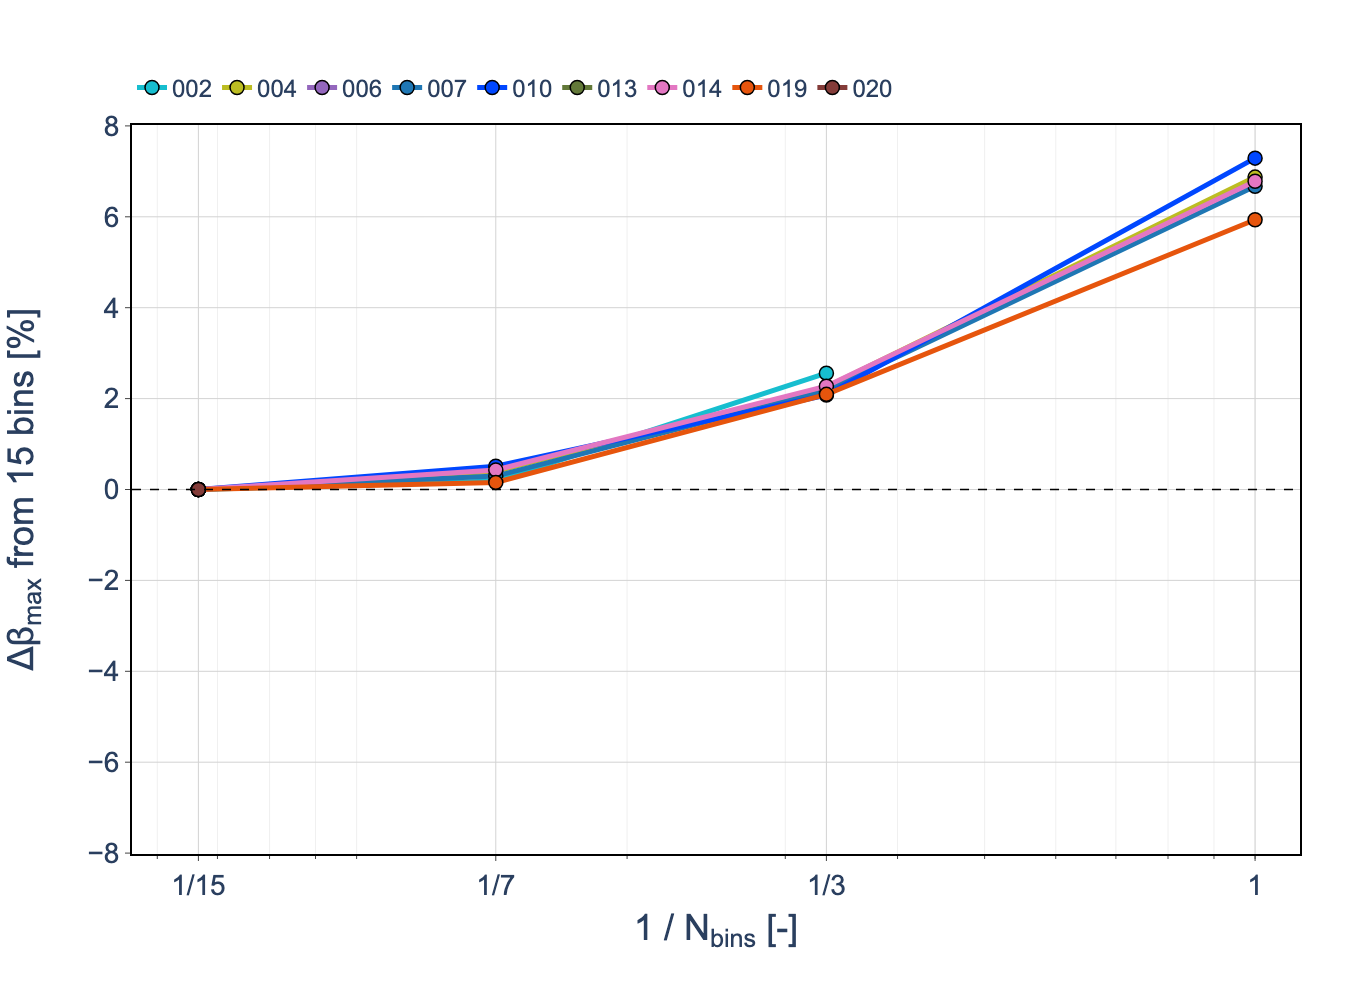
\includegraphics[
        trim={0cm 1cm 1cm 2.6cm},
        clip,
        width=0.98\textwidth
    ]{FIGURES/IMPINGEMENT/tc_naca0012_ae3932_beta_max_distribution_convergence_l1_relative_to_bins15.png}

    \textbf{Relative to 15 Bins}
\end{column}

\end{columns}

\vspace{-0.15cm}

\begin{block}{\scriptsize Observations}
\begin{itemize}
    \item 7- and 15-bin predictions are nearly identical; 3 bins remain within $2$--$3\%$.
    \item A single bin increases $\beta_{\max}$ by approximately $7\%$.
\end{itemize}
\end{block}

\end{frame}


% ============================================================
% Impingement Width -- Grid Convergence
% ============================================================

\begin{frame}{\small Impingement Width Grid Convergence (15 Bins)}
\scriptsize

\vspace{-0.3cm}

\begin{columns}[T,onlytextwidth]

\begin{column}{0.50\textwidth}
    \centering
    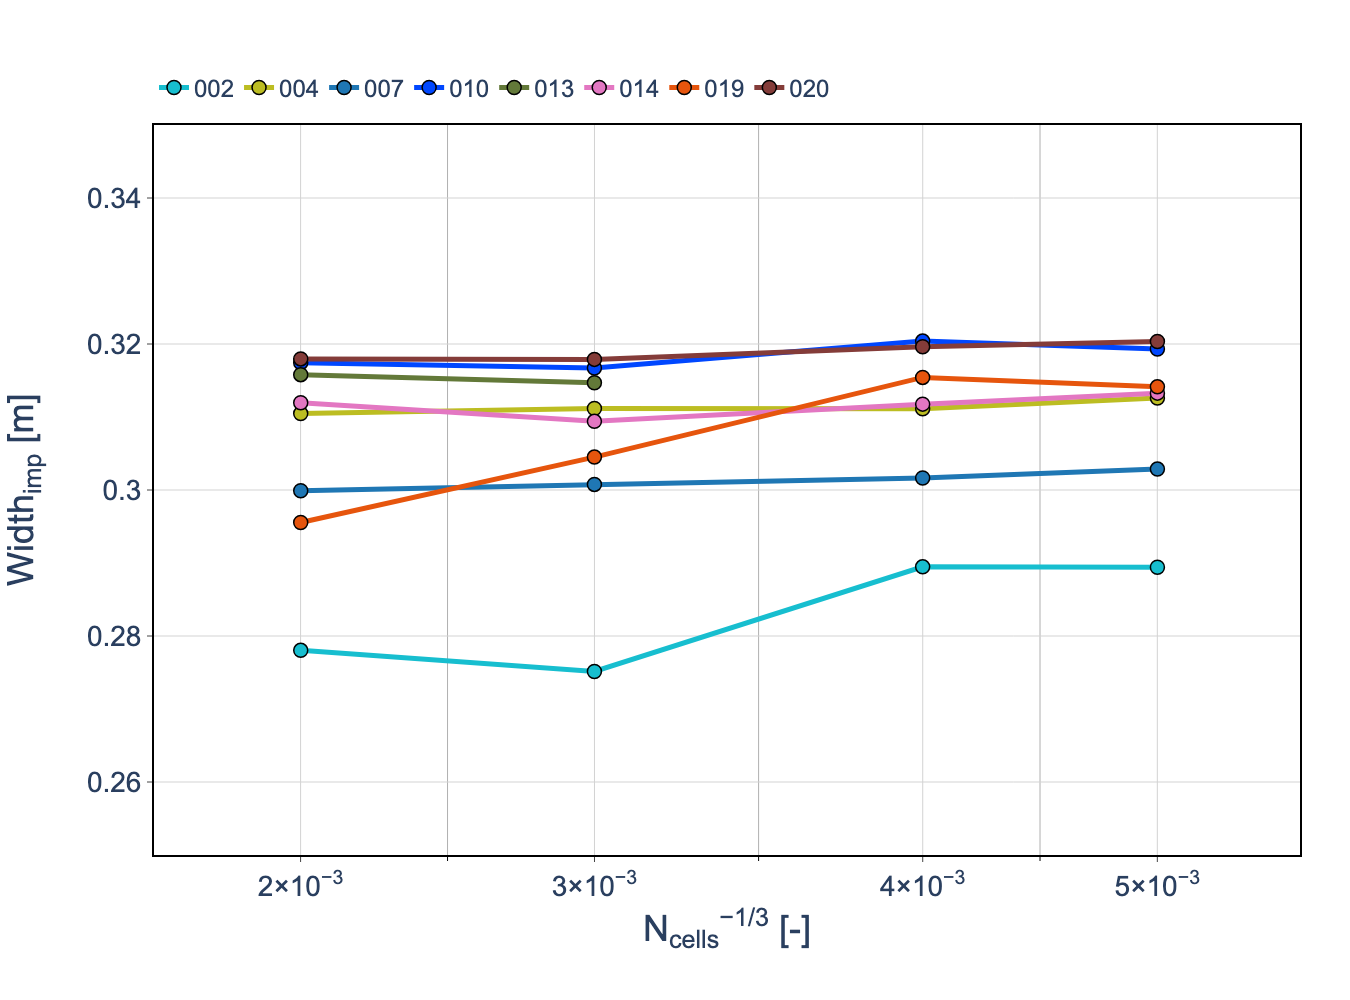
\includegraphics[
        trim={0cm 1cm 1cm 2.6cm},
        clip,
        width=0.98\textwidth
    ]{FIGURES/IMPINGEMENT/tc_naca0012_ae3932_width_bins15.png}

    \textbf{Grid-Level Values}
\end{column}

\begin{column}{0.50\textwidth}
    \centering
    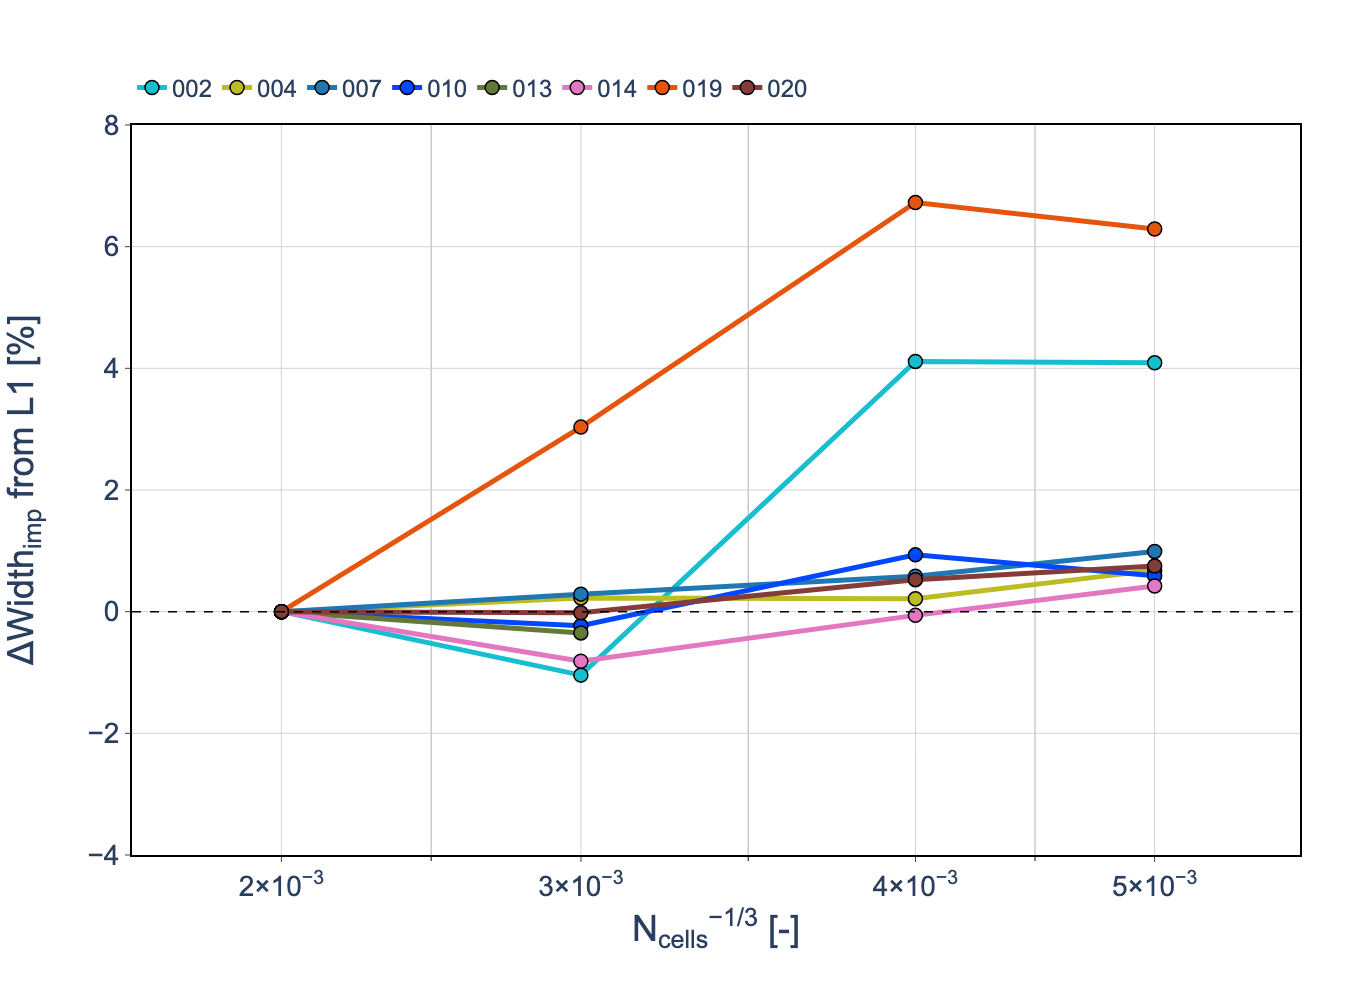
\includegraphics[
        trim={0cm 1cm 1cm 2.6cm},
        clip,
        width=0.98\textwidth
    ]{FIGURES/IMPINGEMENT/tc_naca0012_ae3932_width_bins15_relative_to_l1.png}

    \textbf{Relative to L1}
\end{column}

\end{columns}

\vspace{-0.15cm}

\begin{block}{\scriptsize Observations}
\begin{itemize}
    \item Impingement limits: $\beta=0.0001$ crossings;
    $\mathrm{Width}_{\mathrm{imp}}=s_{\mathrm{upper}}-s_{\mathrm{lower}}$.
    \item At L1, the median impingement width is $0.309~\mathrm{m}$,
    with a $5.4\%$ IQR.
    \item Most grid-level differences remain within approximately $\pm2\%$ of L1,
    with some deviations up to $\sim4-6\%$.
\end{itemize}
\end{block}

\end{frame}


% ============================================================
% Impingement Width -- Droplet-Bin Convergence
% ============================================================

\begin{frame}{\small Impingement Width Droplet-Bin Convergence (L1)}
\scriptsize

\vspace{-0.3cm}

\begin{columns}[T,onlytextwidth]

\begin{column}{0.50\textwidth}
    \centering
    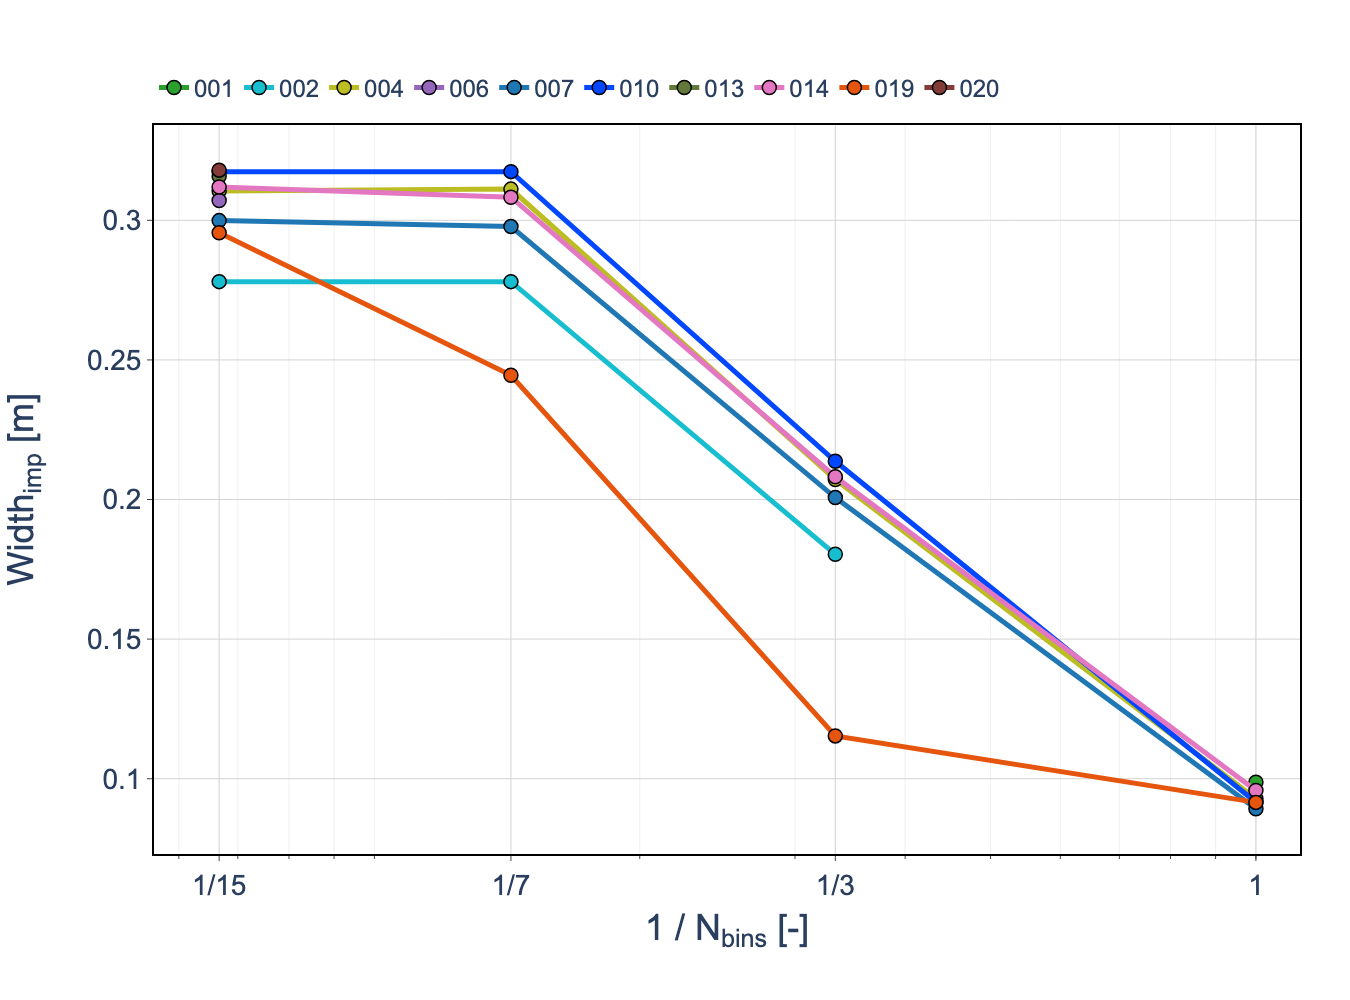
\includegraphics[
        trim={0cm 1cm 1cm 2.6cm},
        clip,
        width=0.98\textwidth
    ]{FIGURES/IMPINGEMENT/tc_naca0012_ae3932_width_distribution_convergence_l1.png}

    \textbf{Bin-Distribution Values}
\end{column}

\begin{column}{0.50\textwidth}
    \centering
    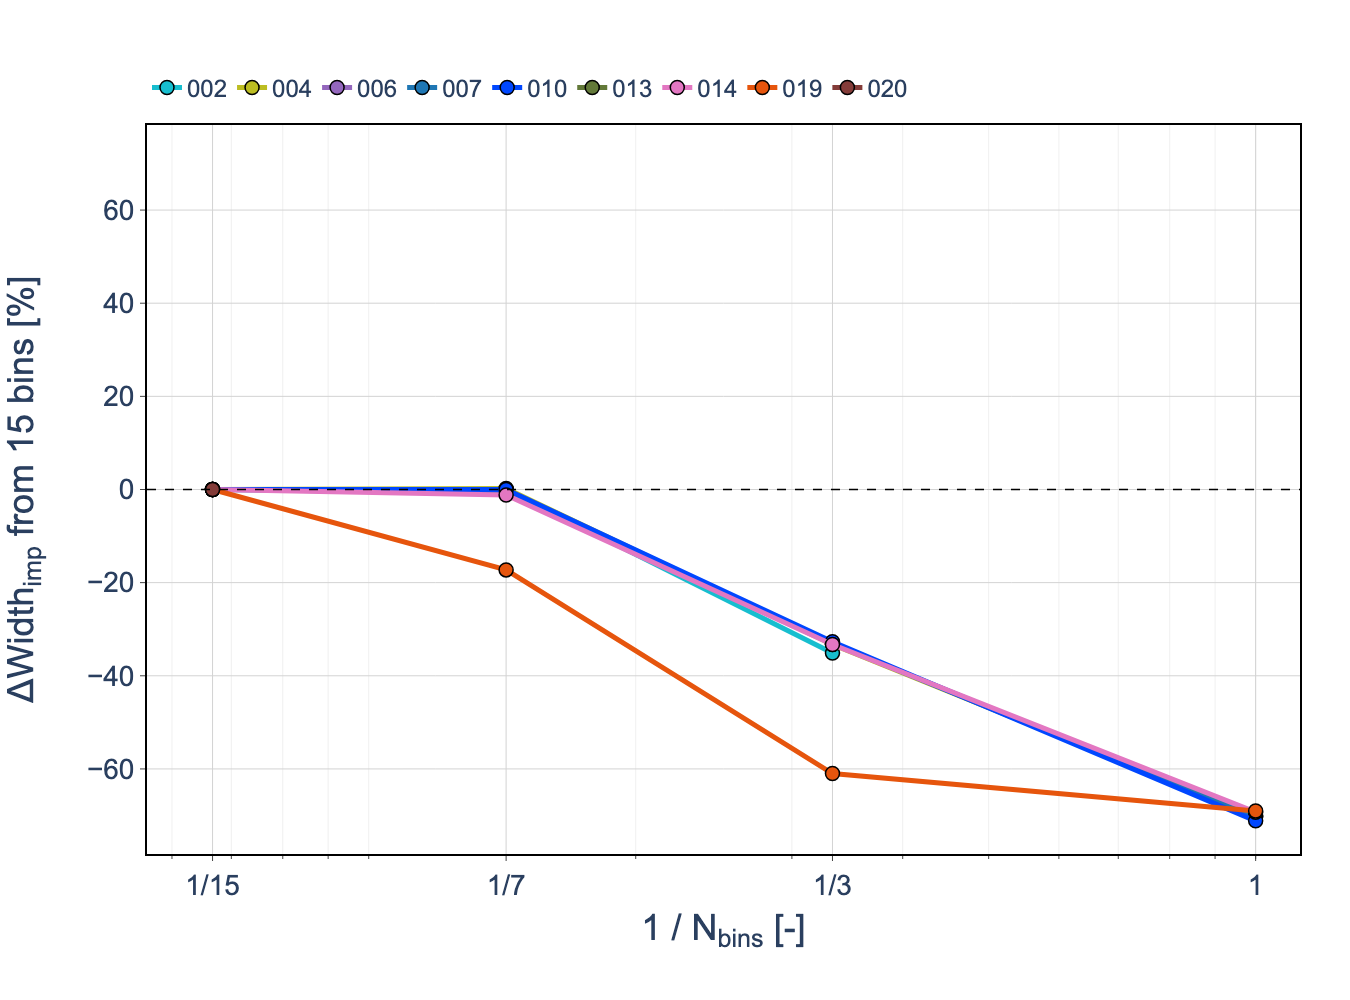
\includegraphics[
        trim={0cm 1cm 1cm 2.6cm},
        clip,
        width=0.98\textwidth
    ]{FIGURES/IMPINGEMENT/tc_naca0012_ae3932_width_distribution_convergence_l1_relative_to_bins15.png}

    \textbf{Relative to 15 Bins}
\end{column}

\end{columns}

\vspace{-0.15cm}

\begin{block}{\scriptsize Observations}
\begin{itemize}
    \item 7 and 15 bins give nearly identical impingement widths ($1-2\%$ difference).
    \item 3 and 1 bin reduce the width by approximately $35\%$ and $70\%$, respectively.
\end{itemize}
\end{block}

\end{frame}


% ============================================================
% Droplet Impingement Assessment
% ============================================================

\begin{frame}{\small Droplet Impingement Assessment}
\scriptsize

\begin{alertblock}{\scriptsize Droplet Impingement Assessment}

\textbf{Spatial Grid Convergence}
\begin{itemize}
    \item Water mass, $\beta_{\max}$, and impingement width show limited grid sensitivity for most submissions.
    
    \item Code-to-code variability is generally comparable to or larger than the grid-refinement effect.
    
    \item Peak position was examined, but its sensitivity to the local leading-edge discretization prevented a clear convergence assessment.
\end{itemize}

\vspace{0.10cm}

\textbf{Droplet-Size Effects}
\begin{itemize}
    \item The 7-bin distribution closely reproduces the 15-bin results, while the single-bin distribution overpredicts $\beta_{\max}$ and underpredicts impingement width and collected water mass.
\end{itemize}

\end{alertblock}

\end{frame}